\documentclass[letterpaper, reqno,11pt]{article}
\usepackage[margin=1.0in]{geometry}
\usepackage{color,latexsym,amsmath,amssymb,graphicx,float,listings,tikz,xcolor}
\usepackage{hyperref}

\hypersetup{
colorlinks=true,
linkcolor=magenta,
filecolor=magenta,
urlcolor=cyan,
}

\lstset{
basicstyle=\ttfamily,
columns=fullflexible,
frame=single,
breaklines=true,
postbreak=\mbox{\textcolor{red}{$\hookrightarrow$}\space},
}

\graphicspath{ {images/} }

\begin{document}

\begin{titlepage}
\newgeometry{margin=2cm}
\centering

\vspace*{\stretch{2}}

\Large Investigation of Michelson Interferometer and Coherence Length

\normalsize

\vspace{\stretch{1}}

% \normalsize Power Supplies and Voltage Regulators

\vspace{\stretch{0.5}}

\begin{tabular}{ll}
Name & Xander Naumenko \\[2ex]
Student number & 38198354 \\[2ex]
Partner & Renu Rajamagesh \\[2ex]
Lab name & Fourier optics \\[2ex]
Lab station  & L2C \\[2ex]
Assigned TA            & Rachel Wang \\[2ex]
Lab \#            & 2 \\[2ex]
Notes &  N/A
\end{tabular}

\vspace{\stretch{1}}

\begin{abstract}
    The Michelson interferometer is a powerful tool capable of accurately measuring extremely small changes in distance. The operating principles of the this device were thoroughly investigated during this lab. Specifically, two main experiments were conducted: the measurement of the exact emission lines of a sodium lamp, and the coherence length of white light. The interferometer was able to experimentally measure the wavelength of a sodium lamp to be 588.8nm, and was able to discern the two lines very close to this wavelength to be within $0.605\pm 0.008$nm of one another. The coherence of white light was found to be approximately $0.27\mu$m.
\end{abstract}

\vspace{\stretch{2}}
\end{titlepage}

\newpage

\section{Research Note}

\subsection{Introduction}

The exact frequencies emitted by a given light source is of great use if the molecular emission spectra are not available. However if multiple emission lines are extremely close together, it can be difficult to separate the two. In this experiment the emission wavelengths of a sodium lamp were investigated.

\subsection{Methods}

A Michelson interferometer works by splitting incoming light and passing it through two arms of different lengths before recombining it. The fringes on this recombined light are caused by the destructive or constructive interference between the split light. By changing the length of one of the arms using a Thor Labs linear slide and measuring how fast the fringes appear and disappear, we recovered the average wavelength of the emitted light. This is possible because one disappearance and reappearance of a fringe corresponds to a $2\pi$ phase shift which occurs every change of path length of size $\lambda$.

However, this only recovers the mean wavelength of the sodium lamp. According to prior research we expect 2 close lines, so to recover the difference between these we measured the contrast of the fringes over a much longer distance. Over long periods the small difference infrequency of the two lines will accumulate to and interfere destructively. Quantitatively, we determined the change in wavelength between the lines using the relation $\Delta\lambda= \frac{\bar\lambda^2}{4d}$, where $d$ is the distance between high and low contrast in the fringes.

\subsection{Results}

Using the methods described above, the mean wavelength of the sodium lamp was determined to be $588.8$nm. The difference between the two lines was determined to be 0.605nm. See figure \ref{fig:rn} for a more detailed picture of the contrast pattern. The generally accepted values for these two parameters is 589nm and 0.5974nm respectively, so these results are consistent with previous investigations into these values.

\begin{figure}[htpb]
    \centering
    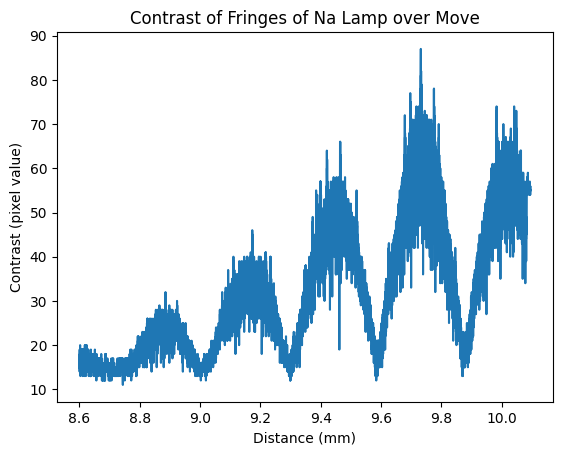
\includegraphics[width=0.5\textwidth]{5B}
    \caption{Fringe contrast for sodium lamp. The main beats are cause by the difference in emission wavelengths of two close lines in the sodium lamp. The increase in amplitude of the contrast over distance is caused by the coherence length, which isn't relevant for emission spectra.}
    \label{fig:rn}
\end{figure}

\newpage

\section{2.3.1: Interference Pattern}

\noindent \textcolor{red}{2.3.1A.} See figure \ref{fig:1A} for the interference pattern observed for both the untilted and tilted mirror. In the untilted case, the waves are reflected perfectly straight from both mirrors, and from the light's perspective there's no difference in any spatial direction. The only variation in path length across the flat coordinates of the camera is the distance from the center $r=\sqrt{x^2+y^2}$ which is of course has circular symmetry. In contrast, when one of the mirrors is tilted then the center of that beam from that mirror doesn't arrive at the center of the image plane. Therefore the interference is no longer as simple, as there is the additional phase of $e^{ik rho^2 /(2R(z))}$ from the Gaussian beam equation. Empirically the tilting of the mirror roughly shifts the fringes.

\begin{figure}[htpb]
    \centering
    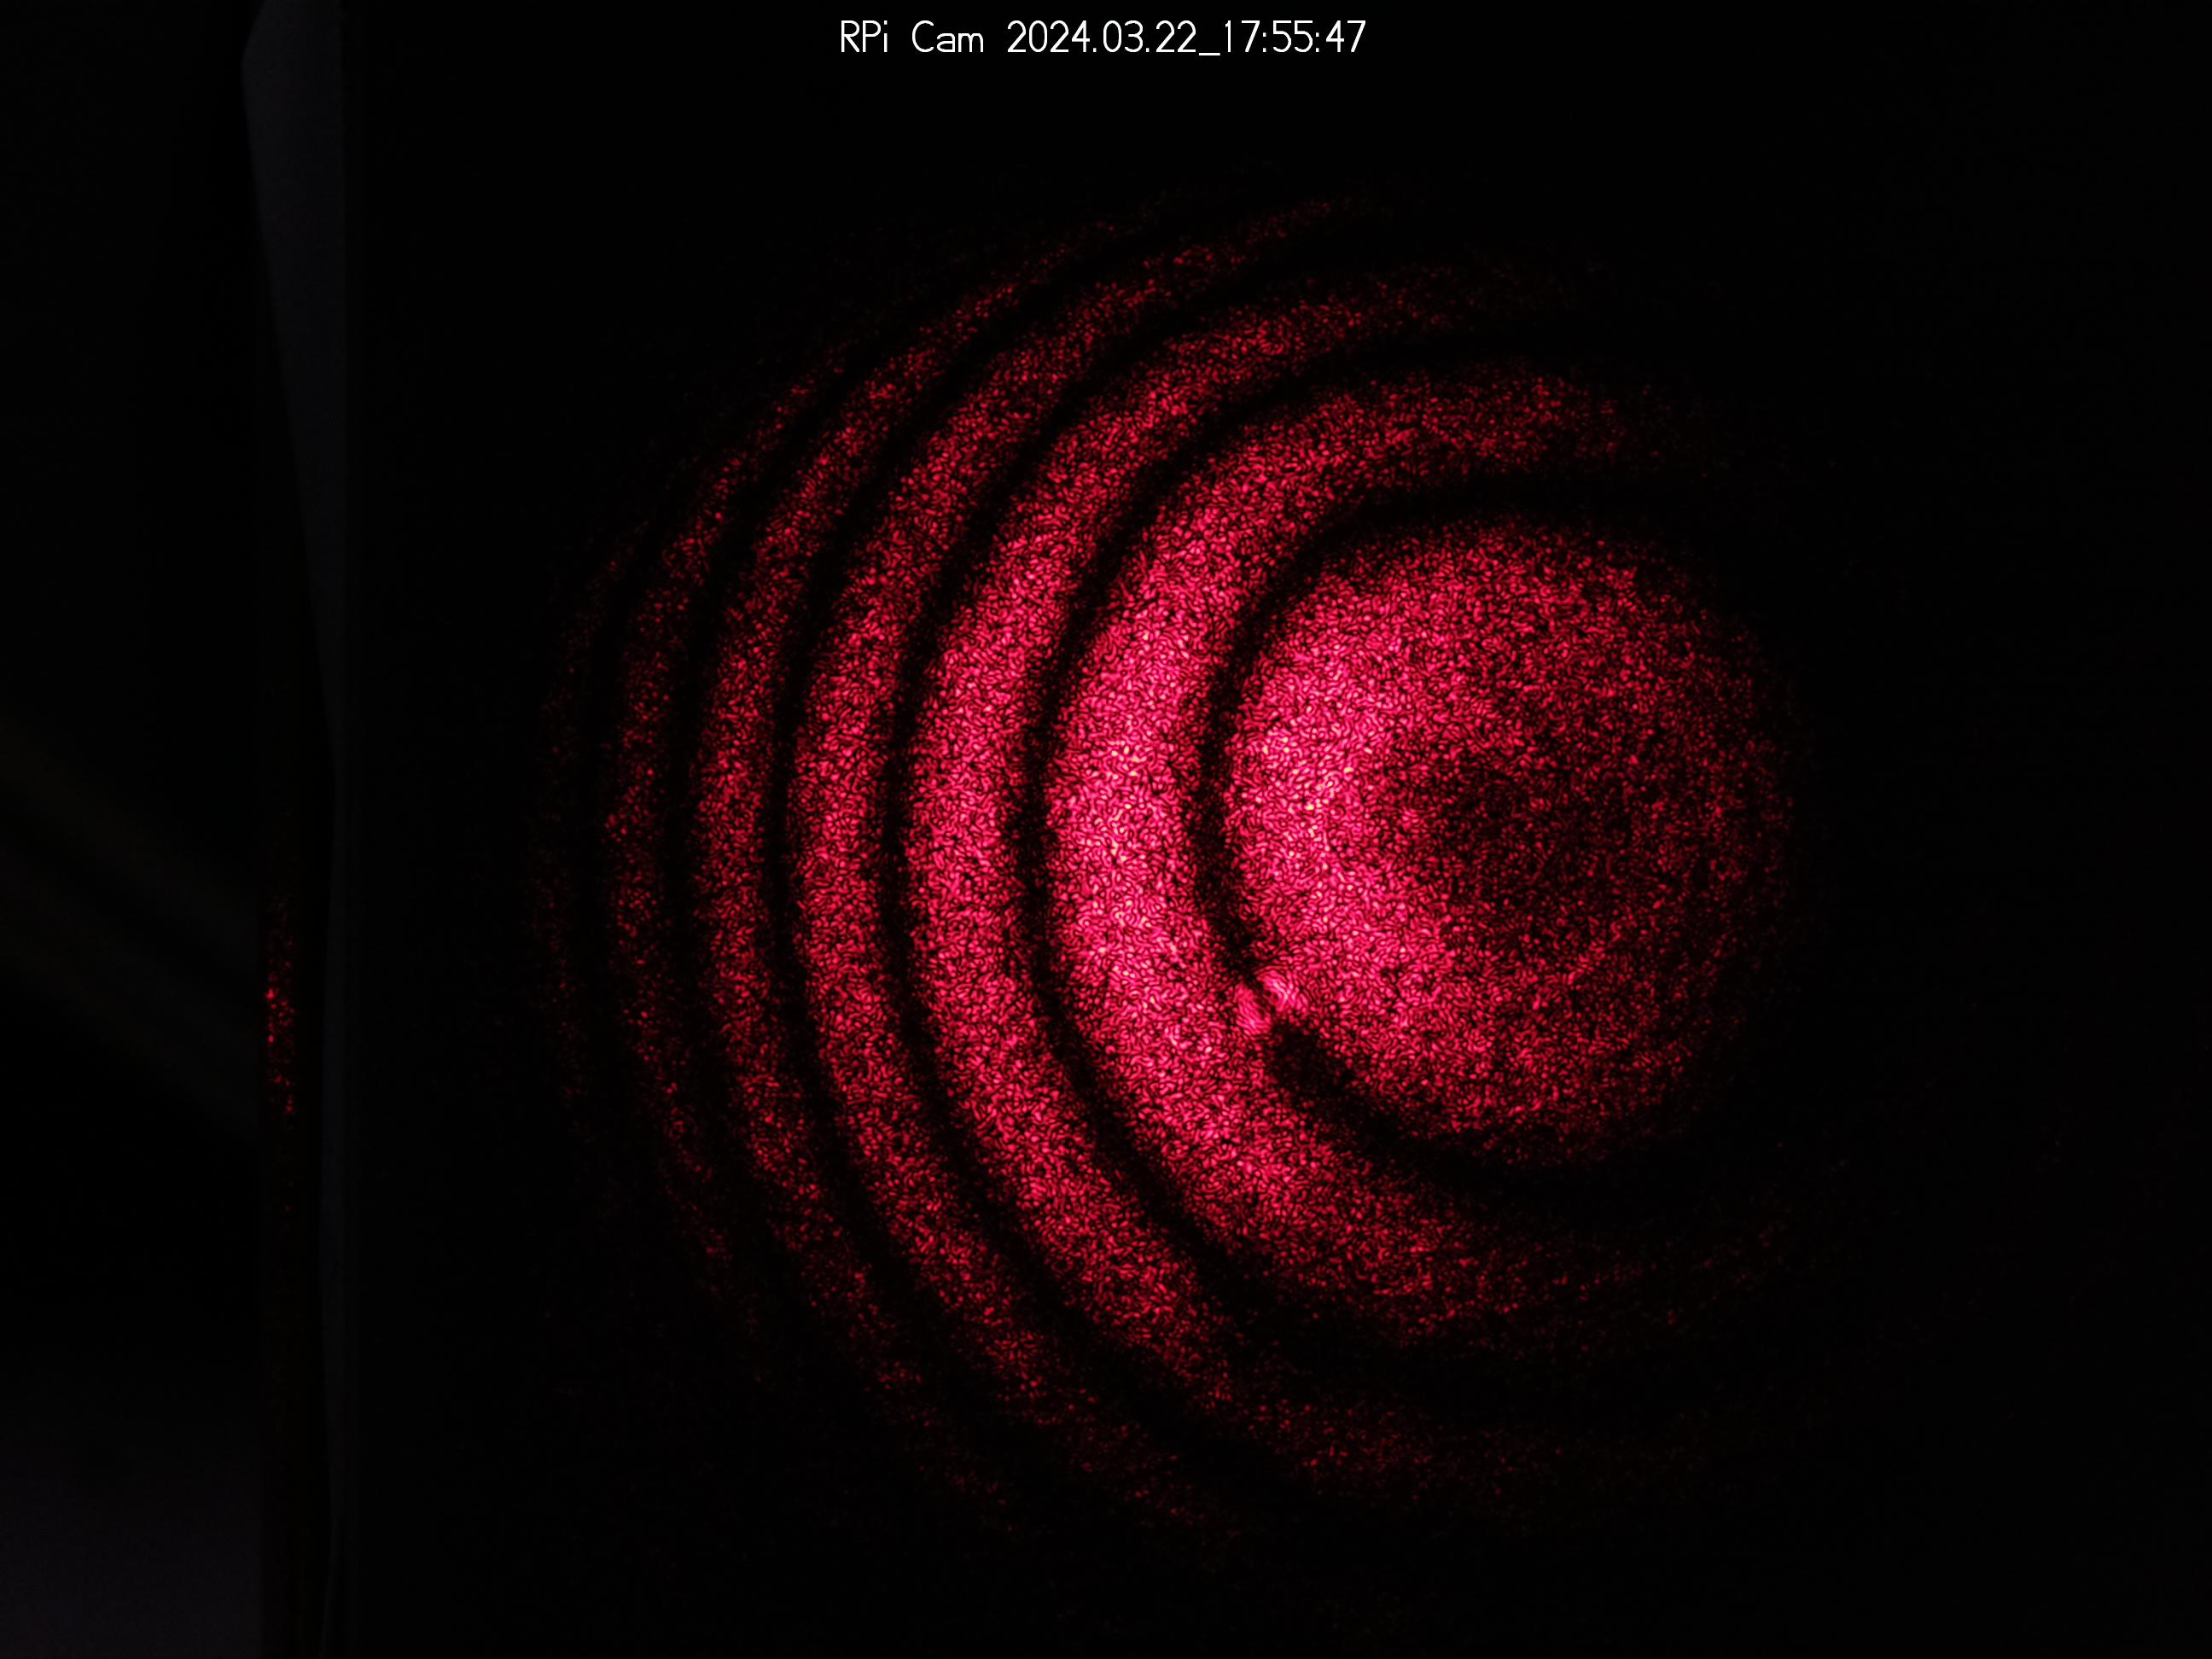
\includegraphics[width=0.49\textwidth]{1A/media/im_0055_20240322_175547.jpg}
    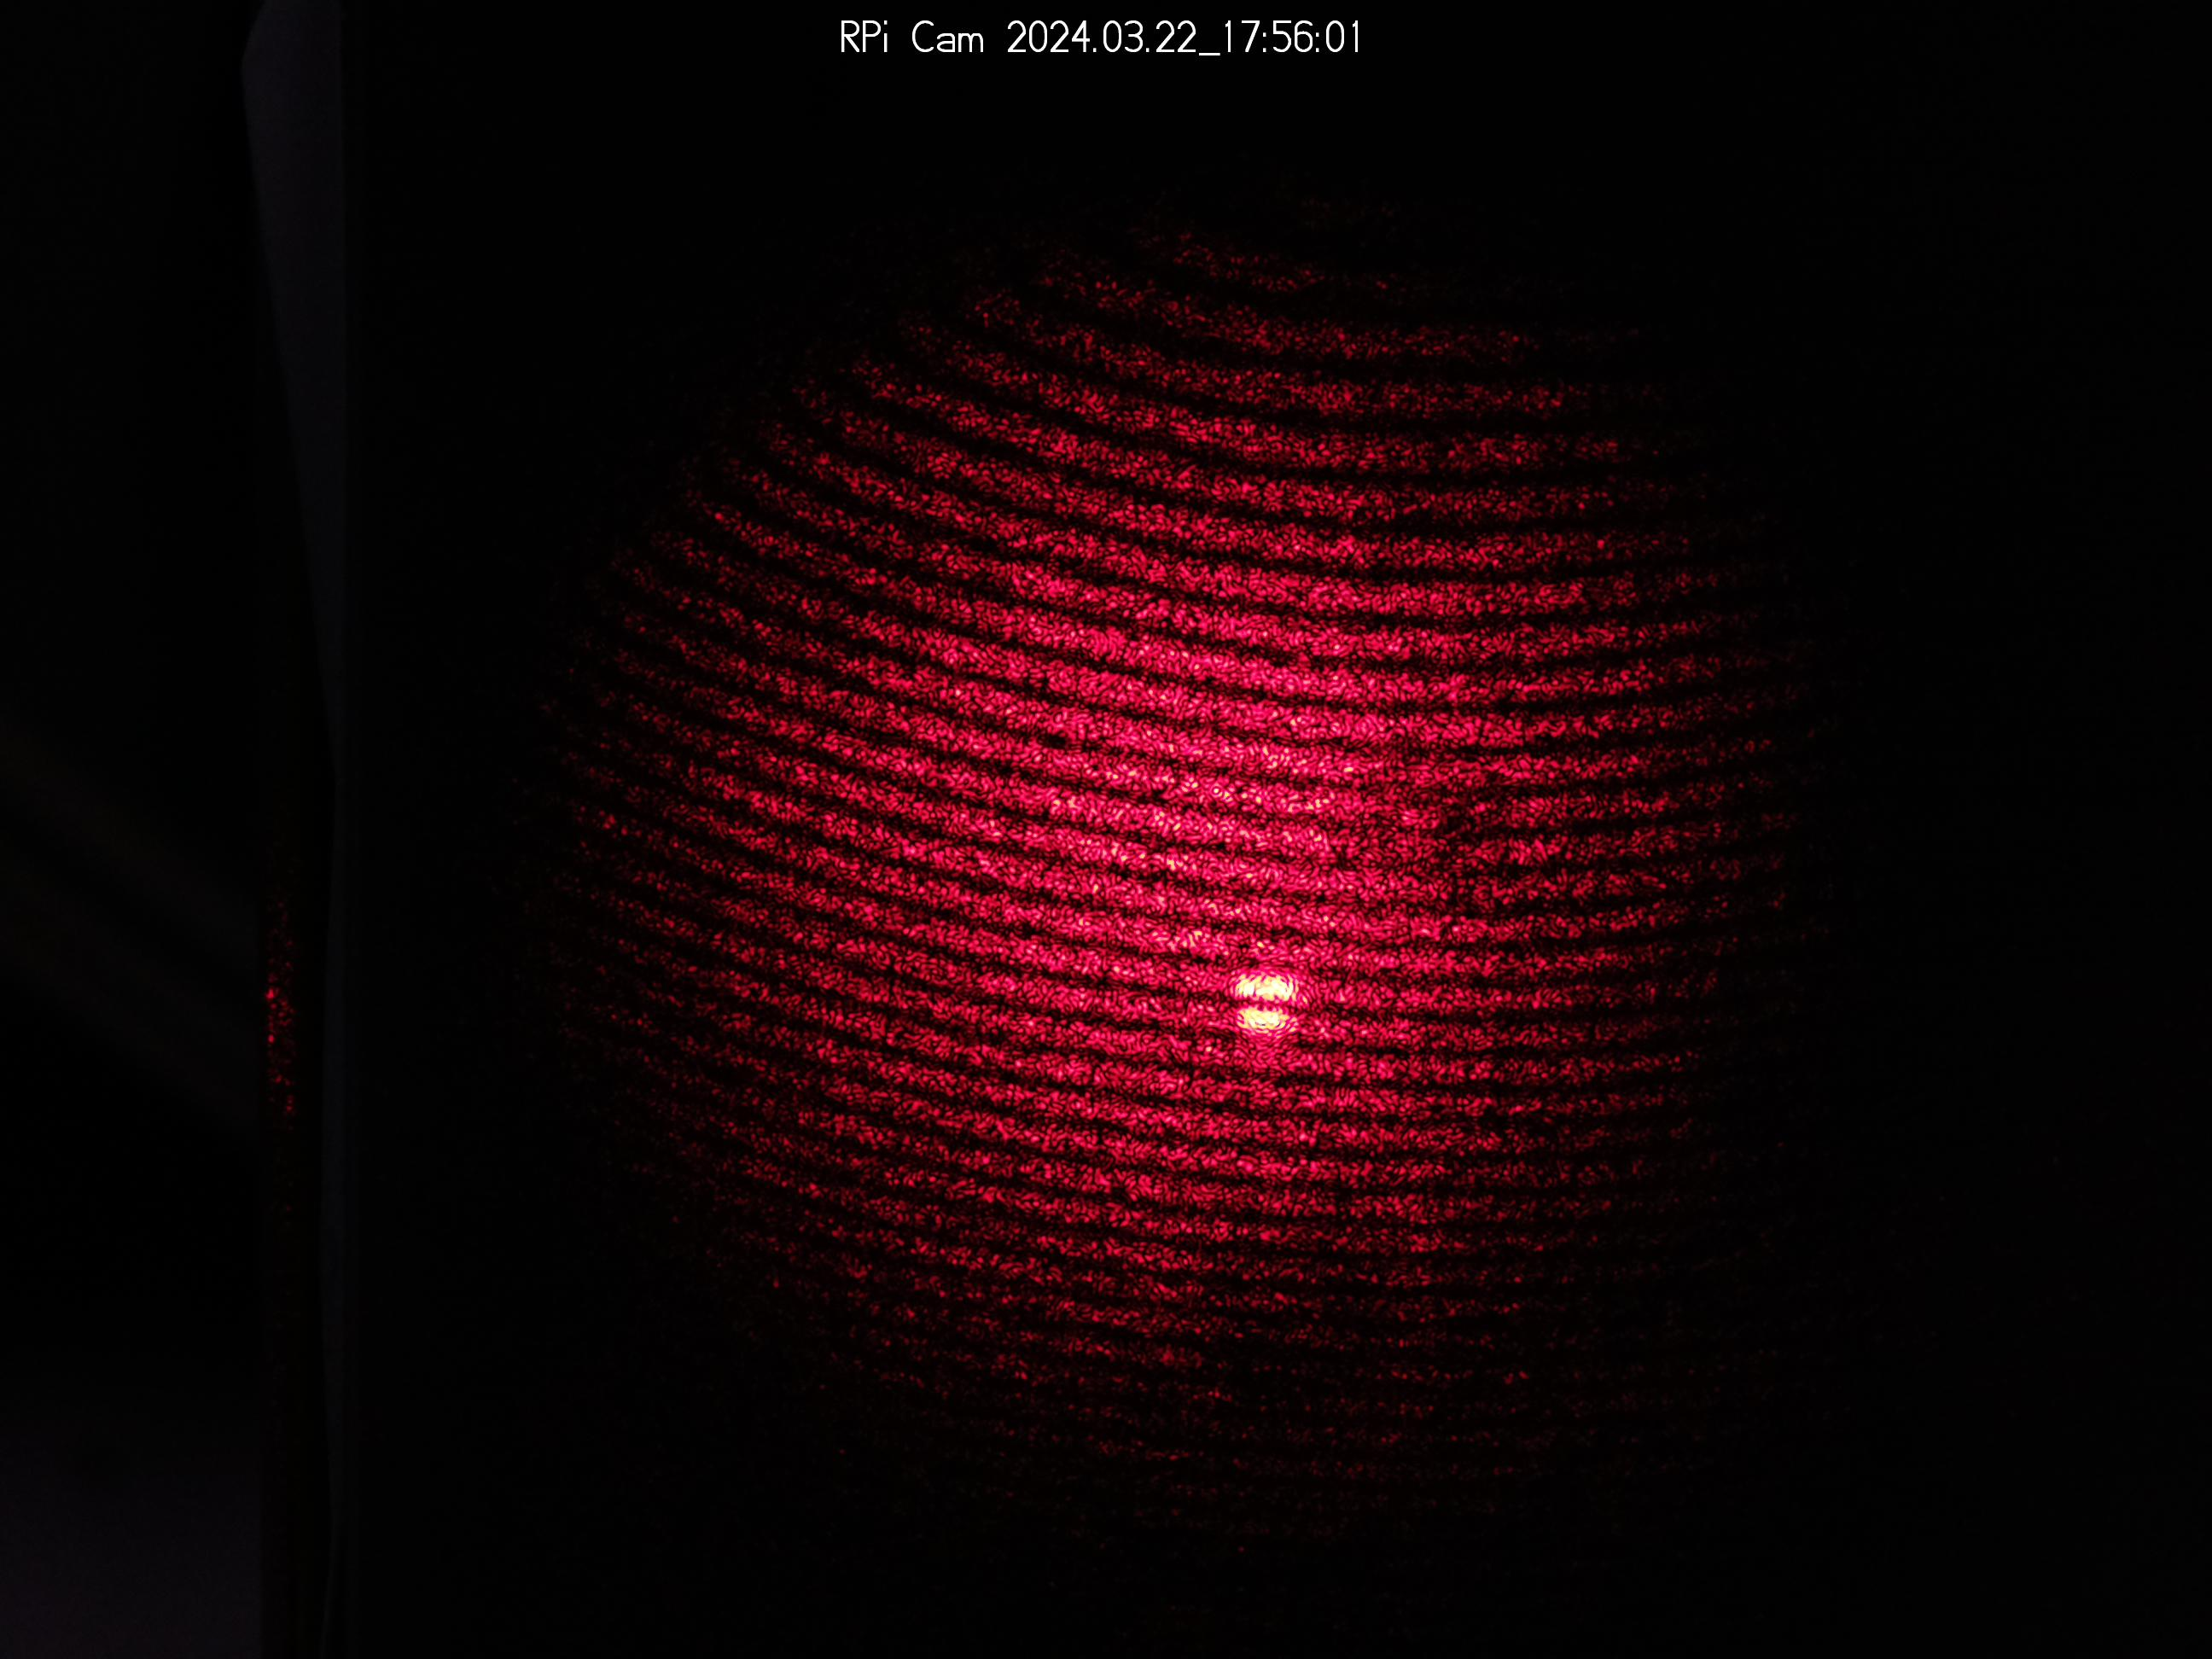
\includegraphics[width=0.49\textwidth]{1A/media/im_0057_20240322_175601.jpg}
    \caption{Interference pattern for 2.3.1A. The fringes occur due to the interference between light from the two different arms of the interferometer with slightly different lengths. Left was captured with no tilt in either mirror, while the right image was captured after a small tilt in the one of the mirrors.}
    \label{fig:1A}
\end{figure}

\section{2.3.2: Index of Refraction of Air}

\noindent \textcolor{red}{2.3.2A.} The beam traverses the cell twice in the interferometer, once forward and the other backwards. The optical path length is thus $\Delta d=20\text{cm}\cdot 2\cdot (n_{\text{air}}-1)=55.4\mu$m, where I'm using a value of $n_{\text{air}}=1.000277$ which I found online. Given that a fringe occurs every $2\pi$ change in phase, the number of fringes that pass is then
\[
N_{\text{fringes}}=\frac{\Delta \phi}{2\pi}= \frac{k\Delta d}{2\pi}=87.55
.\]

\noindent \textcolor{red}{2.3.2B.} The experiment was conducted as described. To convert between frame number and time, we can just just divide the frame counter by the frame rate of the camera, in this case 30. The resulting intensity over time can be seen in figure \ref{fig:2B}. As expected the fringes rapidly oscillate as the air is drained from the chamber. In total there were 65 peaks visible.

\begin{figure}[htpb]
    \centering
    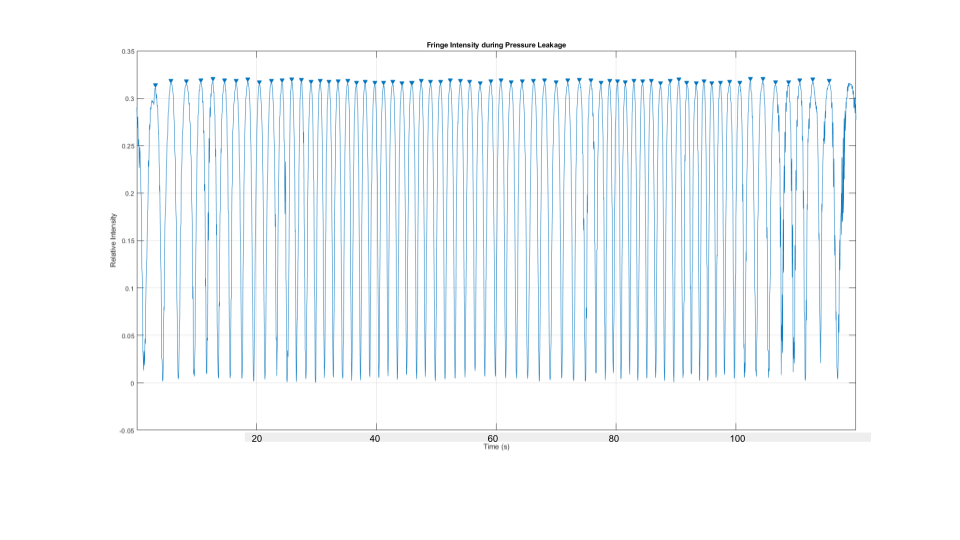
\includegraphics[width=1.0\textwidth]{2B.png}
    \caption{Intensity of a specific point on in the interference pattern as air is drained from the vacuum chamber. The data is truncated to the region where the air is draining, before and after this section the intensity flattens out. The peaks were counted using Matlab's findpeaks function.}
    \label{fig:2B}
\end{figure}

\noindent \textcolor{red}{2.3.2C.} No, we wouldn't have seen the same number. Recall when we calculated the number of fringes above, we used the formula $N_{\text{fringes}}=\frac{k\Delta d}{2\pi}$. Since $k=\frac{2\pi}{\lambda}$ is different between the Na lamp (where $\lambda=589$nm) and the HeNe laser (where $\lambda=632.8$nm). Specifically, we would have seen $N_{\text{fringes}}=\frac{k_{\text{Na}}\Delta d}{2\pi}=94.1$ fringes in that case.

\noindent \textcolor{red}{2.3.2D.} To get our value of $n_{\text{air}}$, we can just follow the calculation for part 2.3.2A backwards:
\[
\Delta d= \frac{N_{\text{fringes}}\cdot 2\pi}{k}\implies n_{air}=1.00019
.\]

This is quite different than the theoretical 1.000277 which is accepted. Of course there are several major sources of error in our calculations. The vacuum pump we used doesn't get to 0 pressure, so the beginning of the counting could have been offset by a few modes. Also we never actually directly measured the length of the vacuum pump and directly took the value of 10cm given in the manual, so this could have been imprecise. Finally, while visually the data looked fine, in principle if air leaks in quickly it's possible that aliasing could occur between the peaks if we opened the pump too far, which would cause peaks to be missed.

\section{2.3.3: Calibrating the Interferometer}

\noindent \textcolor{red}{2.3.3A.} One fringe pass corresponds to a change of path length of $\lambda$. Since the light travels there and back, we have that for one fringe pass, the corresponding distance is
\[
d=\frac{\lambda}{2}=\frac{632.8}{2}=316.4\text{nm}
.\]

\noindent \textcolor{red}{2.3.3B.} To find out the calibration, we want to find what the actual speed that the slide moved at compared to what we commanded it.
\[
    v_{\text{real}}= \frac{N_{\text{fringes}}d}{t}
.\]
For each calibration speed, we can run the slide, count how many fringes go by and plug that into the above equation to get the real speed. This process is repeated 3 times for each speed to get the standard deviation. See table \ref{tab:3B}. Because of time constraints, the same data was used as my lab partner (Renu), which was confirmed to be fine by our lab TA (Rachel). The calibration is within two standard deviations of the commanded speed for both 1 and $3\mu$m/s, however it there is significant different for $5\mu$m/s. 

This is almost certainly due to aliasing of the sampling. This can be seen in a graph of the intensity, such as in figure \ref{fig:3B}. There is only a single point between the peaks and troughs of the intensity, which means we're signaling past the Nyquist frequency (Nyquist requires 2 peaks per period, and each period has 1 peak and 1 trough). This leads to aliasing which is why we see a lower computed speed in our calibration table in table \ref{tab:3B}. In practice this just means we can't get a precise calibration of $v=5\mu$m/s, and so we should refrain from using speeds faster than $3\mu$m/s in future parts.

\begin{table}[htpb]
    \centering
    \caption{Calibration for question 2.3.3B. Note that commanded speed and real speed differ significantly for $5\mu$m/s, this is due to aliasing.}
    \label{tab:3B}
    \begin{tabular}{|c|c|c|}
    \hline
    Commanded Speed ($\mu$m/s) & Real Speed ($\mu$m/s) & Standard deviation, n=3 ($\mu$m/s) \\
    \hline
    1              & 1.06087    & 0.04935            \\
    3              & 2.98486    & 0.01186            \\
    5              & 4.15740    & 0.09265            \\
    \hline
    \end{tabular}
\end{table}

\begin{figure}[htpb]
    \centering
    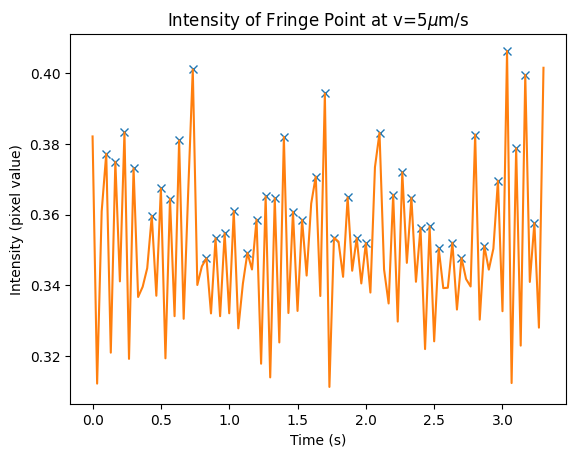
\includegraphics[width=0.5\textwidth]{3B}
    \caption{Intensity of a point over time while moving at $v=5\mu$m/s at a zoomed in time scale to demonstrate aliasing. Peak pattern isn't clear, and occasionally two high points occur next to each other which reduces number of peaks.}
    \label{fig:3B}
\end{figure}

\section{2.3.4: Average Wavelength of the Sodium Lamp}

\noindent \textcolor{red}{2.3.4A.} Since this measurement will take a long time, we want to scan as fast as possible. However as already explained in question 2.3.3B, there is a limit on how fast we can scan since we couldn't calibrate for speeds faster than $3\mu$m/s (see that question and the accompanying figure \ref{fig:3B} for the explanation for why that is). Thus $3\mu$m/s is the optimal speed to conduct the measurement.

\noindent \textcolor{red}{2.3.4B.} The measurement was conducted, see a plot of the measured intensity over time in figure \ref{fig:4B}. The number of peaks measured was 460 over the course of 45.4s. Using these, we can solve for wavelength:
\[
    \lambda = \frac{\Delta d}{N_{\text{fringes}}}=\frac{2v_{real}t}{N_{\text{fringes}}}=588.8\text{nm}
.\]

\begin{figure}[htpb]
    \centering
    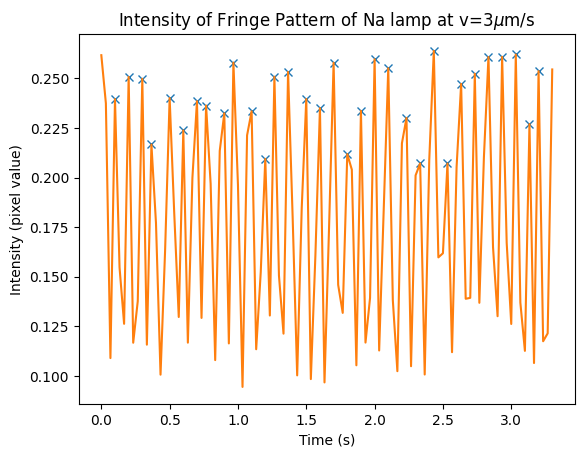
\includegraphics[width=0.5\textwidth]{4B}
    \caption{Intensity over time of sodium lamp. Again similar to figure \ref{fig:3B} this is very zoomed in to be able to see the individual peaks, the actual measurement was conducted over the span of 45.4s. Compare to figure \ref{fig:3B}, the peaks are much more prominent since aliasing isn't as much of a concern.}
    \label{fig:4B}
\end{figure}

\section{2.3.5: Line Splitting of the Sodium Lamp}

\noindent \textcolor{red}{2.3.5A.} To calculate the contrast, we can increase the size of our region of interest and take the difference between the smallest and largest value in it. For the travel distance, we can estimate it by first looking up the real wavelength difference. According to \href{http://hyperphysics.phy-astr.gsu.edu/hbase/phyopt/Na.html}{this} website we expect $\Delta\lambda=0.5974$nm which corresponds to $d_{\text{high}\to\text{low}}=\frac{\bar \lambda^2}{4\Delta\lambda}=0.1445$mm. Since we want to see several peaks, a reasonable distance to scan would be 1.5mm. Finally for speed, from the same logic as described in question 2.3.4A, it makes most sense to use $3\mu$m/s. The hint suggests doing something more clever, but due to the logistics it wasn't inconvenient to run a slightly longer scan so the entire scan was done using $3\mu$m/s.

\noindent \textcolor{red}{2.3.5B.} See figure \ref{fig:5B}. To get as accurate of a result for $d_{\text{high}\to\text{low}}$ as possible, we take the difference between the first minimum of the graph ($9.015\pm 0.005$mm) and the last ($9.875\pm 0.005$mm) and divide by the number of high to low transitions in between (6). The uncertainty of the minimums was estimated from the resolution of the measurements. This gives $d_{\text{high}\to\text{low}}=0.143\pm 0.001$. From this we can calculate $\Delta\lambda=\frac{\bar \lambda^2}{4d_{\text{high}\to\text{low}}}=0.605\pm 0.008$nm.

The theoretical value was already found online in part A to be $0.5974$nm. This is within uncertainty of the experimental value seen.

\begin{figure}[htpb]
    \centering
    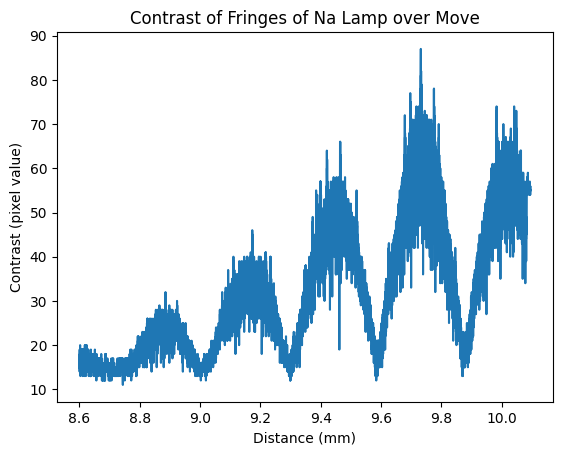
\includegraphics[width=0.5\textwidth]{5B}
    \caption{Contrast of fringes of the sodium lamp over the course of its move at speed $3\mu$m/s. }
    \label{fig:5B}
\end{figure}

\section{2.3.6: Coherence Length of White Light}

\noindent \textcolor{red}{2.3.6A.} Although the question suggests retaking the data from part 2.3.5 in case the table was bumped, to avoid taking extraneous data we first tried searching for the ZPL around the point we saw last week. From this we estimated the ZPL to be at approximately 9.7492mm, as this is near the highest of figure \ref{fig:5B} and when jogging the slide manually this was the point with the largest radius of curvature.

The reason the radius of curvature is largest at the ZPL is that, by definition, it is the point where the two path lengths are the exact same. At any other point there will be at least a small amount of incoherence between the light from the two arms of the interferometer, causing more interference and thus tighter fringes.

\noindent \textcolor{red}{2.3.6B.} Luckily, as soon as we switched out the lamp we immediately saw fringes from the white light, so the filter wasn't actually necessary. Regardless, we also experimented with the filter to see the effect of the wider window. See figure \ref{fig:6B} for the resultant plot. Note that the question asks for intensity but both for this question and the next, however instead we chose to record contrast. This is because what we actually want is the width of the high contrast region, which is when fringes appear. The intensity gives a fine grained view of the how fast the individual fringes move which isn't relevant in this case.

The plot has a half amplitude width, and thus coherence length of $21\mu$m. The reason that we see a much wider range is that the coherence length is inversely proportional to the frequency range. The filter restricts the frequency range to a much narrower band, so as a result the coherence length increases. Note that even though it's an improvement over white light, the filter is nowhere near as good as the sodium lamp. This implies that the window of light the filter passes is much wider than the very strict 598nm we saw for the Na lamp.

\begin{figure}[htpb]
    \centering
    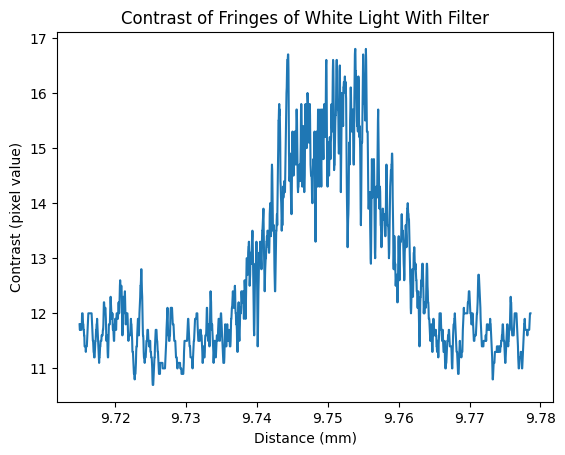
\includegraphics[width=0.5\textwidth]{6B}
    \caption{Fringe contrast of white light with 598nm filter. Note a moving average filter with width 10 was applied, as the discretisatie of pixel values made it difficult to see otherwise.}
    \label{fig:6B}
\end{figure}

\noindent \textcolor{red}{2.3.6C.} See figure \ref{fig:6C}. From this data, we find the half amplitude width to be $2.7\mu$m. This is close to the $3\mu$m we expect from white light. It is a much shorter coherence length than with the filter. This makes sense though, since white light has a much larger bandwidth.

\begin{figure}[htpb]
    \centering
    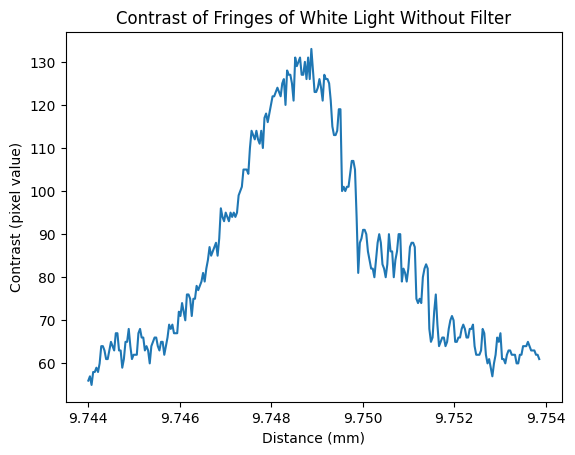
\includegraphics[width=0.8\textwidth]{6C}
    \caption{Contrast plot for fringes of unfiltered white light.}
    \label{fig:6C}
\end{figure}


\end{document}
